We need to have a fairly dense beam of our target species to reach the ion trap center in order to get a reasonable signal to noise of the cold molecule reaction as opposed to the warm background reactions. A dense beam coupled with good cryopumping ensures that the signals seen are primarily, if not solely due to the introduction of the cold beam.

The downstream properties of a beam all start with the buffer gas stagnation density within the experimental cell. The stagnation density is the steady state buffer gas density that is determined by the physical dimensions of the cell, including the aperture, and the gas throughput, or number flow rate going in. Experimentally, it's preferable to use volumetric flow rates when operating the apparatus, so for calculations, that needs to translate to number flow rate using the ideal gas law:

\begin{equation*}
	\dot{N} = \frac{P f}{k_B T}
\end{equation*}

where $P$ is pressure and $f$ is the volumetric flow rate, this translates to about $4\times10^{17}$particles/s$^{-1}$ for 1 SCCM of gas flow. By solving for the number density in the flow out of an aperture with molecular flow, we find that the stagnation density within the cell can be shown as:

\begin{align}
	C_{ap} & = A \frac{\bar{v}}{4} \nonumber \\
%	\frac{\dot{N}}{n_b} & =  A \frac{\bar{v}}{4} \nonumber \\ 
	n_{b} & = \frac{4 \dot{N}}{A_{aperture} \bar{v}} \label{eq: n_b}
\end{align}

In general, buffer gas beams operate with stagnation densities around $10^{15}-10^{17}$cm$^{-3}$. Outside of the cell, we can describe the density of the beam as a function of distance. \cite{Pauly}

\begin{equation}
	n(z)=\frac{n_0}{2}\left(1-\frac{z}{\sqrt{z^2+a^2}}\right)
	\label{eq: n(z)}
\end{equation}

Where $z$ is the distance from the aperture into the vacuum side, $n_0$ is the initial number density, $a$ is the radius of the aperture. In the far-field, this goes to:

\begin{equation*}
	n(z)=\frac{n_0 a^2}{4 z^2}
\end{equation*}

But there is something that we must consider, that is that we aren't seeing the full aperture while we are at all locations, we are actually seeing an appended area due to the inclusion of apertures and skimmers in the way. While only $n_0$ is only dependent on the aperture size of the cell, $n(z)$ will have a set value defined by the smallest aperture in the beam path. For us, although our cell aperture is $\approx$ 9 mm in diameter, we have multiple apertures and skimmers in the way, the smallest of which is a skimmer from Beam Dynamics with a diameter of 2 mm.

Sympathetic cooling occurs through collisions between the hot target species being introduced and the cryogenic buffer gas particles. We may consider each hard sphere collision to transfer heat from the hot target species ($T_s$) to the cold buffer gas at constant temperature ($T_b$).

\begin{equation*}
	\Delta T_s = -\frac{T_s - T_b}{k}
\end{equation*}

Where $k \equiv \frac{(m_b + m_s)^2}{2 m_b m_s}$. For the $N^{\text{th}}$ collision, we can write the change in temperature:

\begin{equation*}
	T_s(N) - T_s(N-1) = -\frac{T_s(N-1)-T_b}{k}
\end{equation*}

For large values of $N$, where the change in temperature becomes small, we can turn the discrete equations into a differential form.

\begin{equation*}
	\frac{d T_s(N)}{dN} = -\frac{T_s(N) - T_b}{k}
\end{equation*}

Which we can solve with the condition that $T_s(0)=T_0$
\begin{align*}
%	T_s(N) & = (T_0 - T_b)e^{-N/k} +T_b \\
	\frac{T_s(N)}{T_b} & = \left(\frac{T_0}{T_b} - 1\right)e^{-\frac{N}{k}} +1 \\
	& \approx \frac{T_0}{T_b}e^{-\frac{N}{k}} + 1
\end{align*}

Assuming an ablation loading process in which $T_0=1 \times 10^4$ K, we find that it still only takes $\approx 12$ collisions to thermalize the target species within a factor of 2 of the buffer gas temperature. In general $\approx 100$ collisions are needed to relax rotational states to the same range.\todo{cite this?} Vibrational degrees of freedom may take upwards of $10^4$ collisions to fully thermalize if the elastic collision energy is much lower than the internal vibrational level.

By finding the mean free path, we can consider the characteristic length the particles travel to be thermalized with the buffer gas, this is then compared to the characteristic length of the cell to determine the effectiveness of the cooling.

\begin{equation*}
	\lambda = \frac{A_{aperture} \bar{v}}{4 f \sigma \sqrt{m_s/m_b}}
\end{equation*}

If a species is introduced into the buffer gas cell that has a lower vapor pressure than that is allowed at the current temperature, it will be lost when it comes in contact with the cell walls. The rate of this loss can be described as the  characteristic time of diffusion of a particle in the buffer gas to the physical dimensions of the cell set the diffusion time constant:

\begin{equation}
	\tau_{diff} = \frac{16}{9 \pi} \frac{A_{cell} n_{0,b} \sigma}{\bar{v}} \label{eq: tau_diff}
\end{equation}

where $\sigma$ represents the collisional cross section for the buffer gas with the target species. On the other hand, we have the characteristic pump out time given by the conductance of a cell aperture:

\begin{equation}
	\tau_{pump}=\frac{4V_{cell}}{\bar{v}A_{aperture}} \label{eq: tau_pump}
\end{equation}

By combining equations \cref{eq: tau_diff,eq: tau_pump}, we can get a dimensionless ratio, $\gamma$ that characterizes the extraction fraction out of the cell.

\begin{equation}
	\gamma = \frac{\tau_{diff}}{\tau_{pump}} = \frac{\sigma f}{L_{cell} \bar{v}} \label{eq: gamma}
\end{equation}

Notice that the $\gamma$ factor does not depend on aperture size, this is generally true, but increasing the aperture size will lower your number density within the cell, which then influences the characteristic length scale of thermalization. Larger apertures thus run the risk of not allowing your particles to fully thermalize in rotational/vibrational states. But decreasing the aperture size can make alignment as well as controlling the number density more difficult, as finer control over the flow rate is necessary for equivalent flow regimes.

Using equations \cref{eq: gamma,eq: n_b}, knowing the physical dimensions of the experimental cell, we find that we may derive theoretical characteristics of the buffer gas beam. During normal operation, our main control over the buffer gas beam is the manipulation of the Ne flow rate, so as a function of buffer gas flow rate ($f$), we may see how key properties are affected.

\begin{figure}[H]
	\centering
	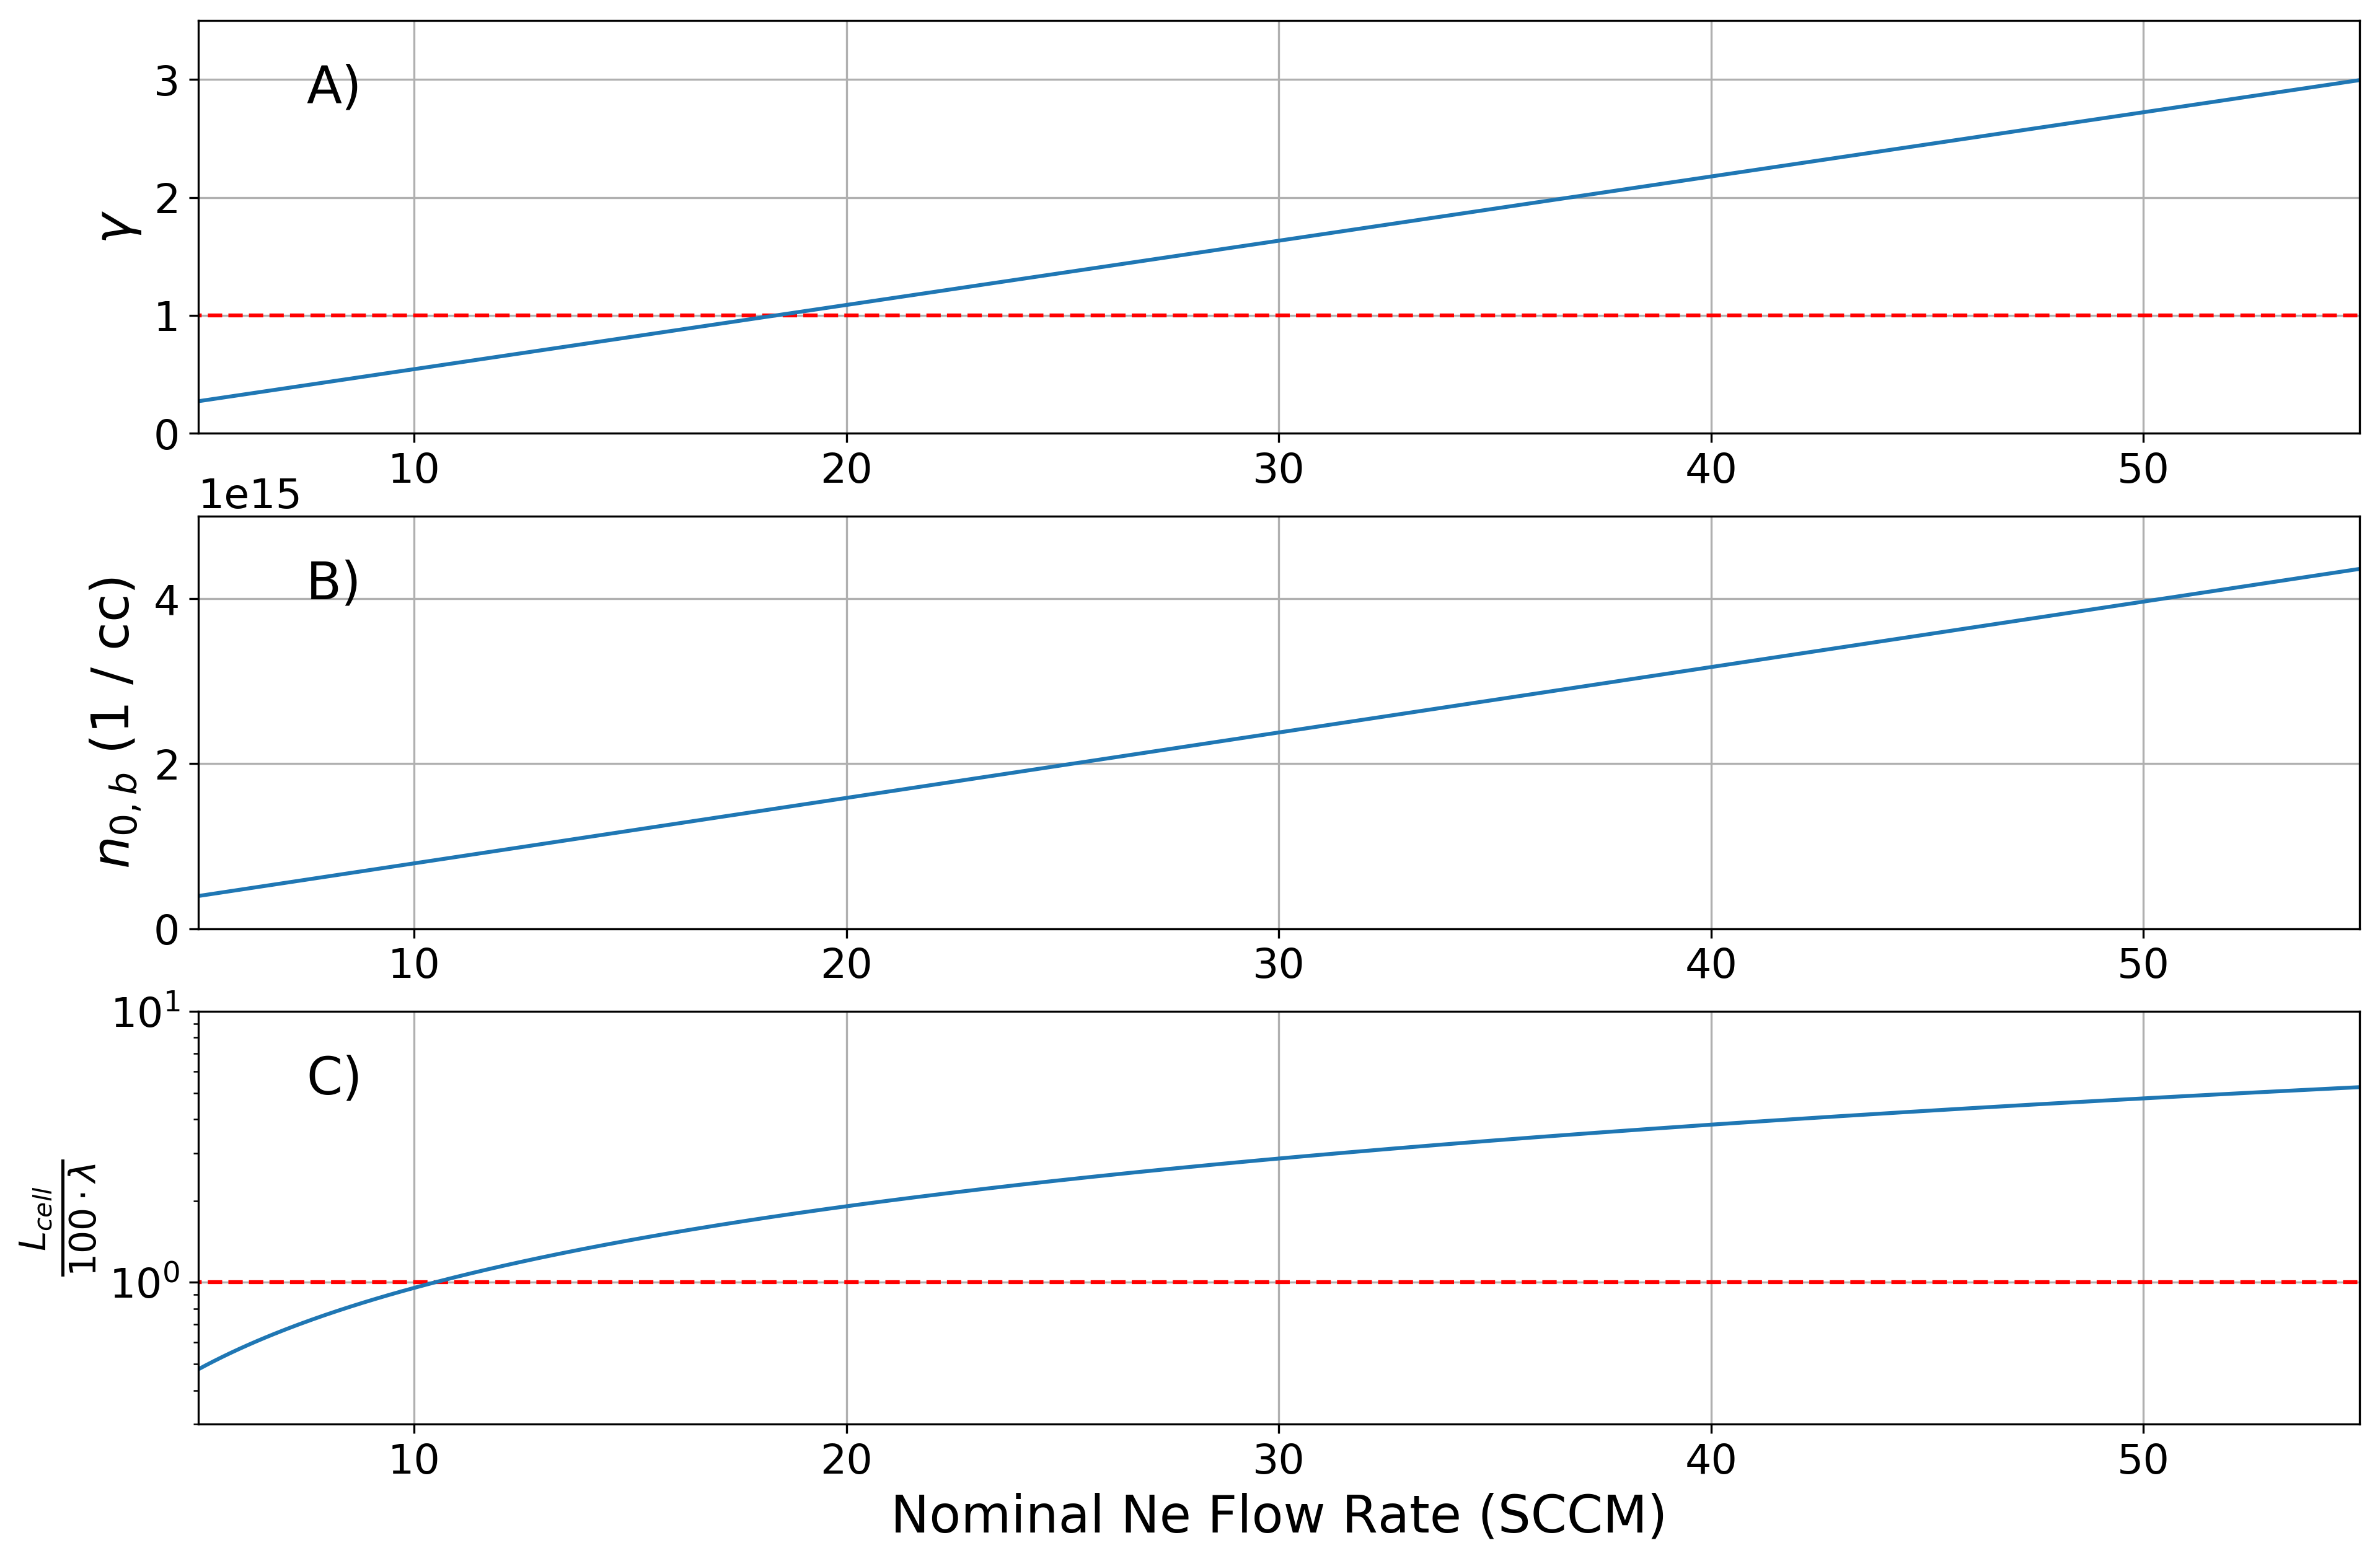
\includegraphics[width=1\textwidth]{images/CBGB_flow_characteristics.png}
	\caption{Theoretically derived buffer gas beam properties of interest given the physical dimensions of our cell in particular: $d_{aperture} = 9$ mm. A) $\gamma$ extraction ratio, dotted red line indicates $\gamma = 1$ where hydrodynamic entrainment begins. B) Number density of buffer gas species within the experimental cell, given an enclosed back wall. The density of target species introduced should stay under 1\% of the buffer gas density for other properties to hold. C) Number of collisions a target species particle would expect before extraction out of the cell, the dotted red line indicates 100 collisions before extraction, when rotational degrees of freedom are characteristically thermalized.}
	\label{fig: buffer_gas_flow}
\end{figure}

\subsection{Direct density measurements}

Although we can make statements about the properties of the buffer gas itself in the beam, we are most interested in the properties of the target species introduced into the cell. In particular, understanding the extraction ratio $\gamma$, as well as the velocity, gives us a good handle on the target species characteristics.

To observe the extraction of the target species from the cell, a residual gas analyzer (RGA) is used to determine the density of the beam in the ballistic regime upstream from the ion trap. To ensure the highest possible signal, the Swagelok vernier flow valve used to regulate water vapor flow into the cell is fully opened. During normal operation of the beam in conjunction with the ion trap, the valve is set to a much smaller opening to ensure the properties of the beam are dominated by the buffer gas species, as well as to control the reaction rates.

\begin{figure}[H]
	\centering
	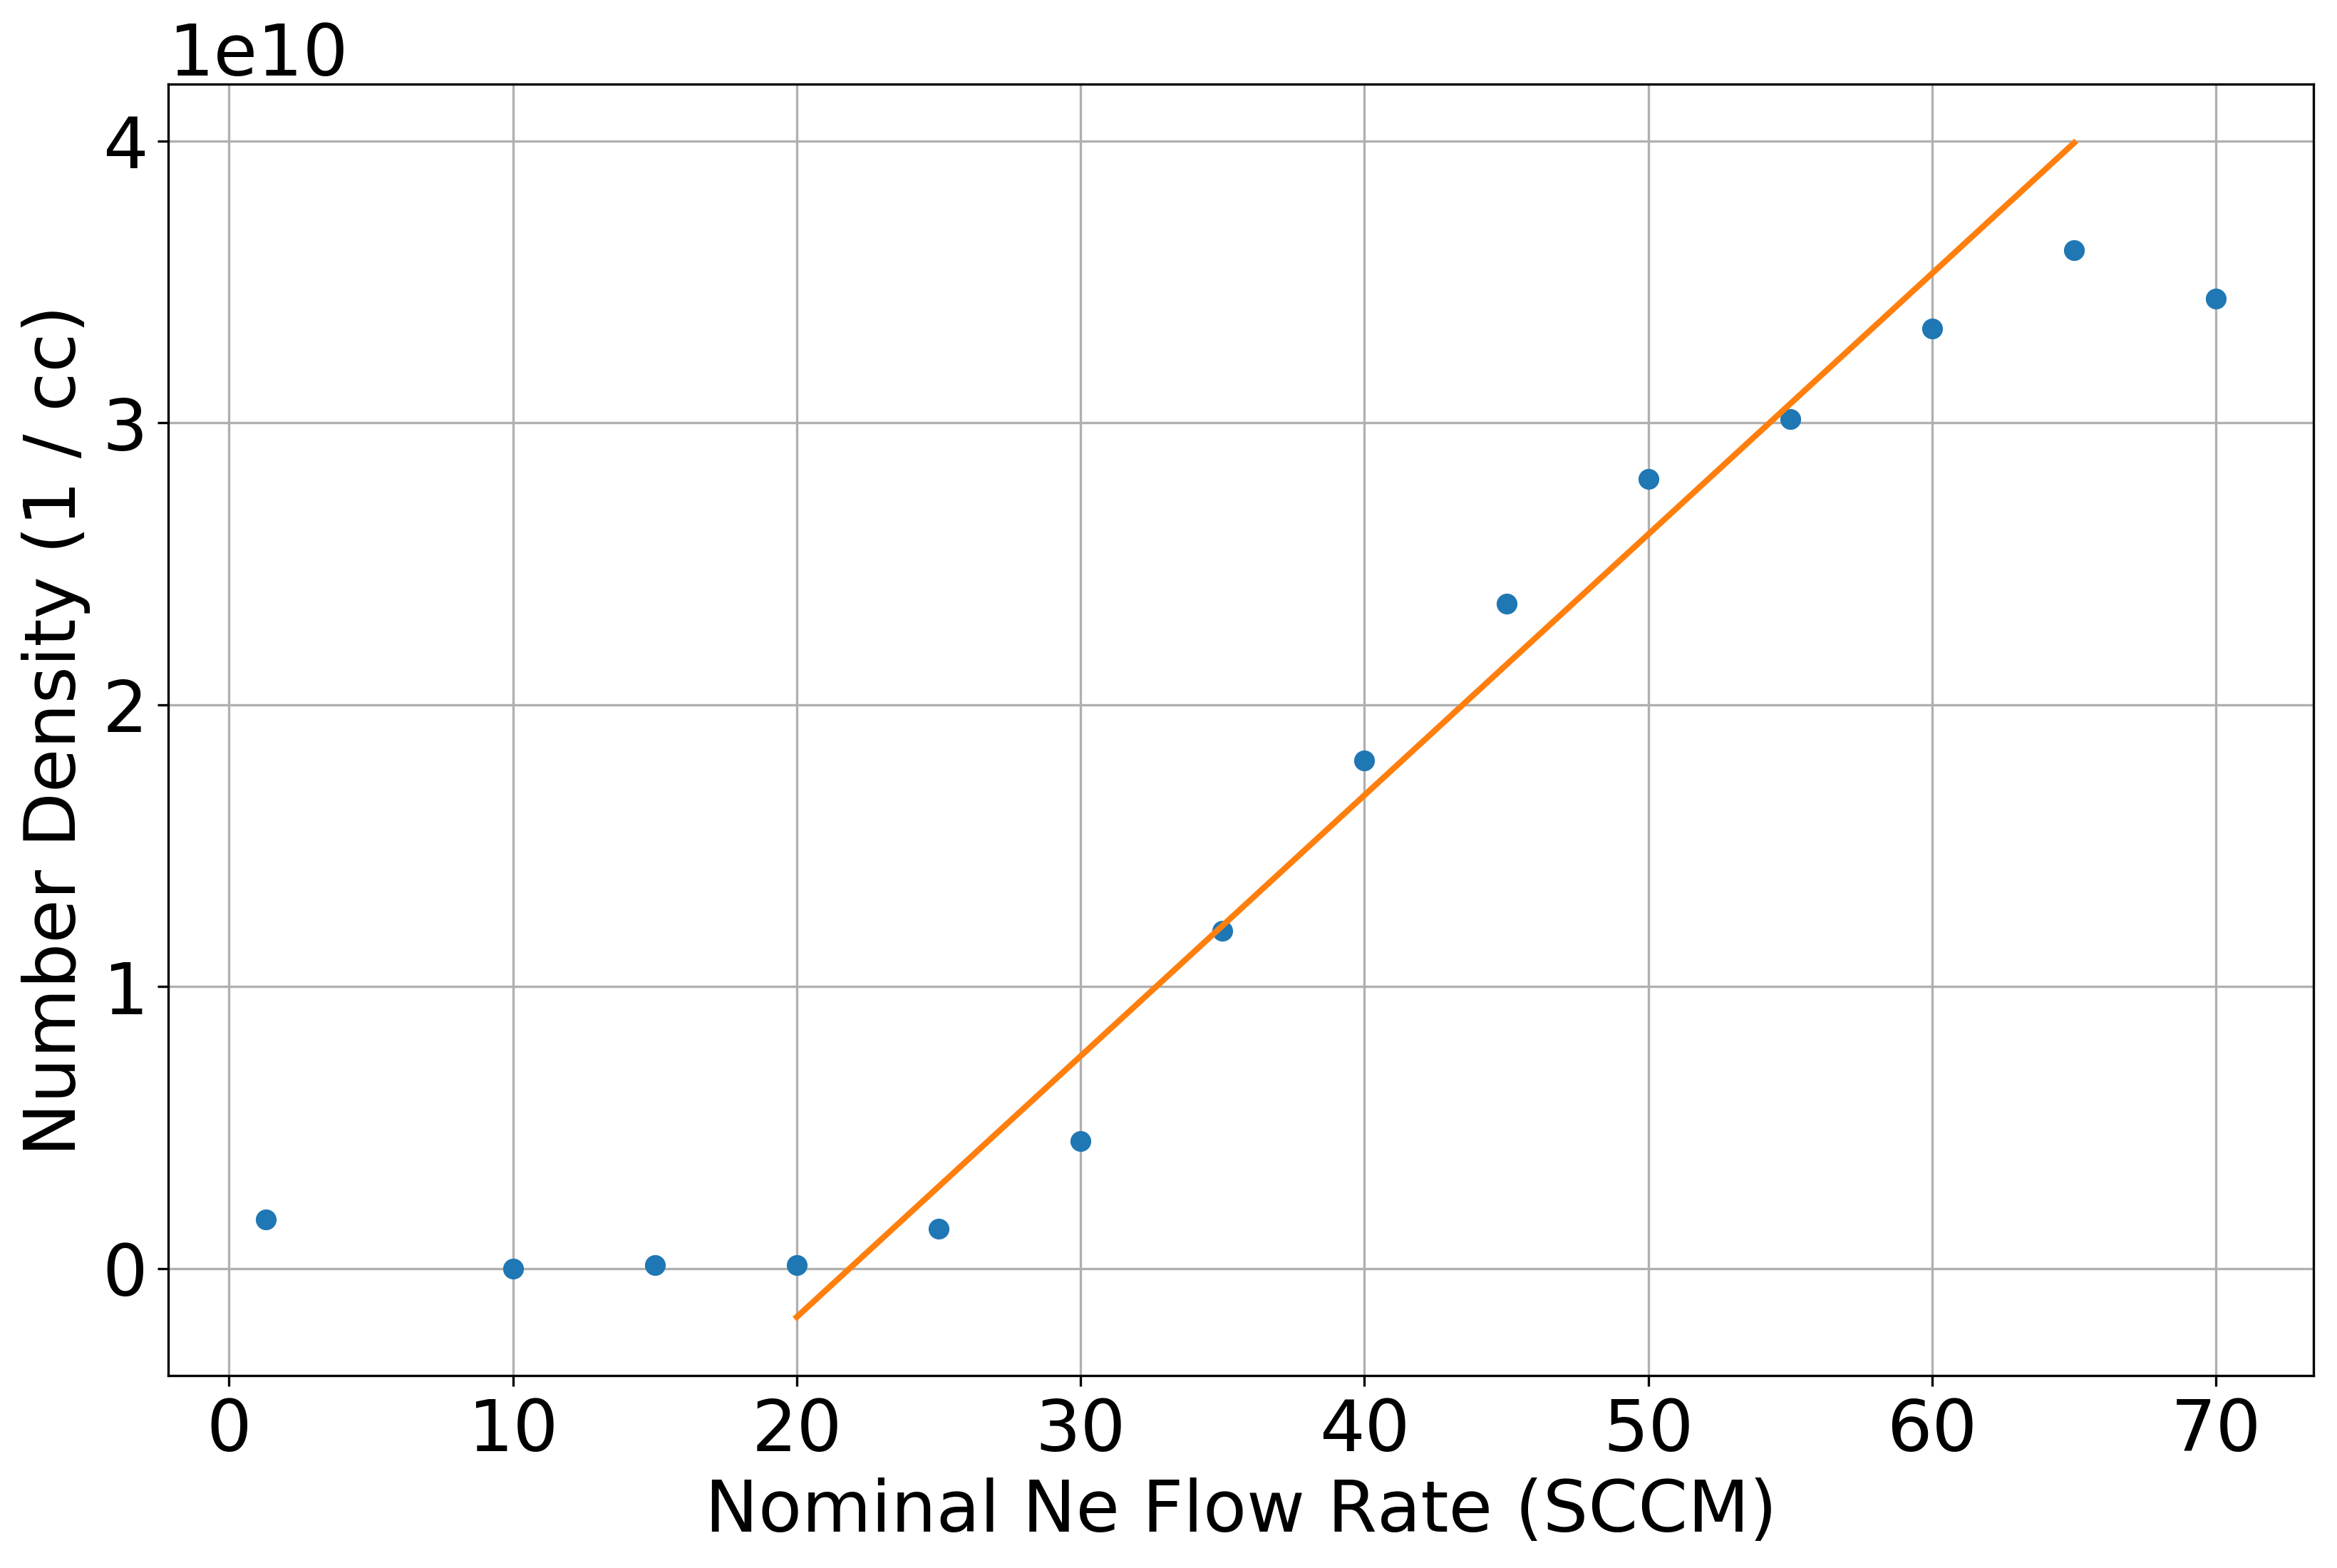
\includegraphics[width=0.8\textwidth]{images/CBGB_hydrodynamic_fit.png}
	\caption{Fitted linear behavior of \ce{H2O} entrained in a \ce{Ne} buffer gas beam 30 cm from cell aperture. The onset of hydrodynamic entrainment seems to occur around 20 SCCM up through 60/65 SCCM where the \ce{H2O} extracted into the beam has a clear linear form of ($9.2 \times 10^8$ cm$^{-3}$/SCCM)$f - 2 \times 10^{10}$ cm$^{-3}$.}
	\label{fig: rga entrainment}
\end{figure}

We find that theoretical calculations and experimental results agree that the onset of hydrodynamic entrainment occurs at a buffer gas flow rate of $\approx$ 20 SCCM. We can combine the results here with equations \cref{eq: mb_mean,eq: n_b,eq: n(z)} to map out beam densities subject to all other possible parameters we may want to adjust, over our entire experimental apparatus. We start by scaling a combination of equations \cref{eq: n_b,eq: n(z)} by $\alpha$, a buffer gas to target species density scaling factor.

\begin{equation*}
	n(z) = \alpha\frac{f}{A_{aperture} \bar{v}}\left(1-\frac{z}{\sqrt{z^2+a^2}}\right)
\end{equation*}

But this only holds true for the region in which the number density is linearly dependent to the buffer gas flow rate, not over all possible ranges; we've seen that the target species only behaves linearly in the hydrodynamic regime. This means that we should be equating the function of $n(z)$ with the linear fit performed on the data for the parameters the data was taken at.

\begin{equation*}
	mf+b = \alpha\frac{f}{A_{aperture, 0} \bar{v_0}}\left(1-\frac{z_0}{\sqrt{z_0^2+a_0^2}}\right) 
\end{equation*}

Where $z_0=30$ cm, being the distance of the RGA from the cell aperture, and $z=0=2$ mm, for the smallest aperture seen during the experimental run. We also define the experimental scaling factors:

\begin{align*}
	\alpha & = \frac{m}{\beta}+\frac{b}{\beta f} \\
	\beta & = \frac{1}{A_{aperture, 0} \bar{v_0}}\left(1-\frac{z_0}{\sqrt{z_0^2+a_0^2}}\right)
\end{align*}

Thus, we obtain a form that includes experimentally derived scaling factors that allows us to project the target species density over the length of the system.

\begin{equation}
	n(z) = \frac{mf+b}{A_{aperture} \bar{v} \beta}\left(1-\frac{z}{\sqrt{z^2+a^2}}\right)
	\label{eq: experimental n(z)}
\end{equation}

\begin{figure}[H]
	\centering
	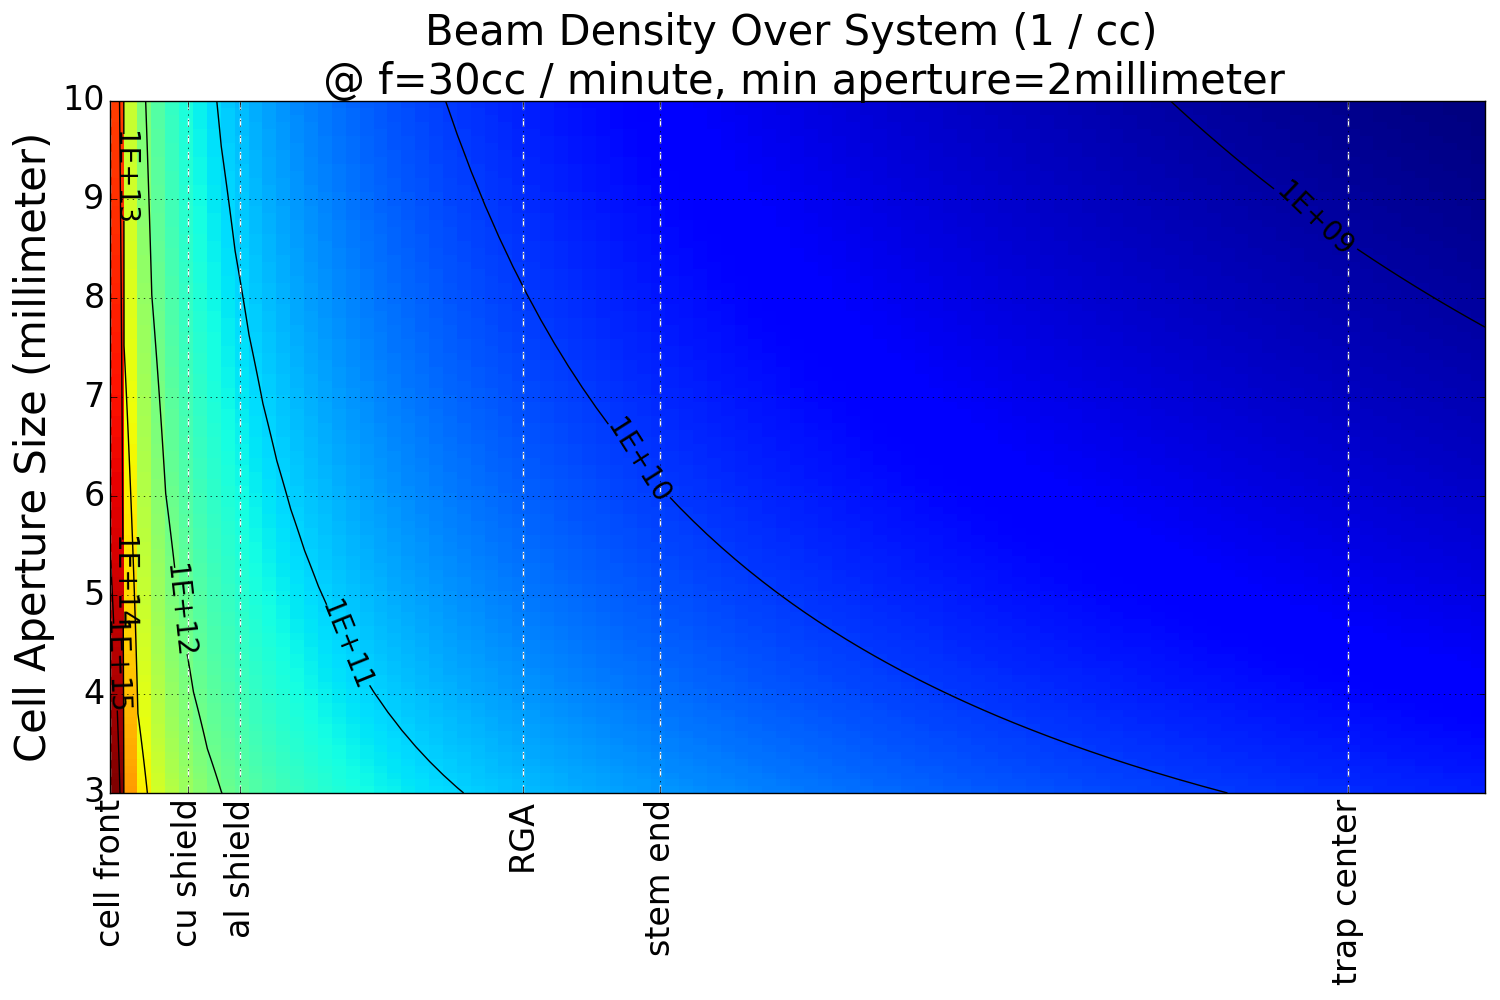
\includegraphics[width=1\textwidth]{images/CBGB_beam_density_over_system.png}
	\caption{Projected beam densities with a Ne flow rate of 30 SCCM with various distances of interest within the chamber. Beam densities shown are without throttling of the \ce{H2O} flow valve.}
	\label{fig: beam_density}
\end{figure}

\begin{figure}[H]
	\centering
	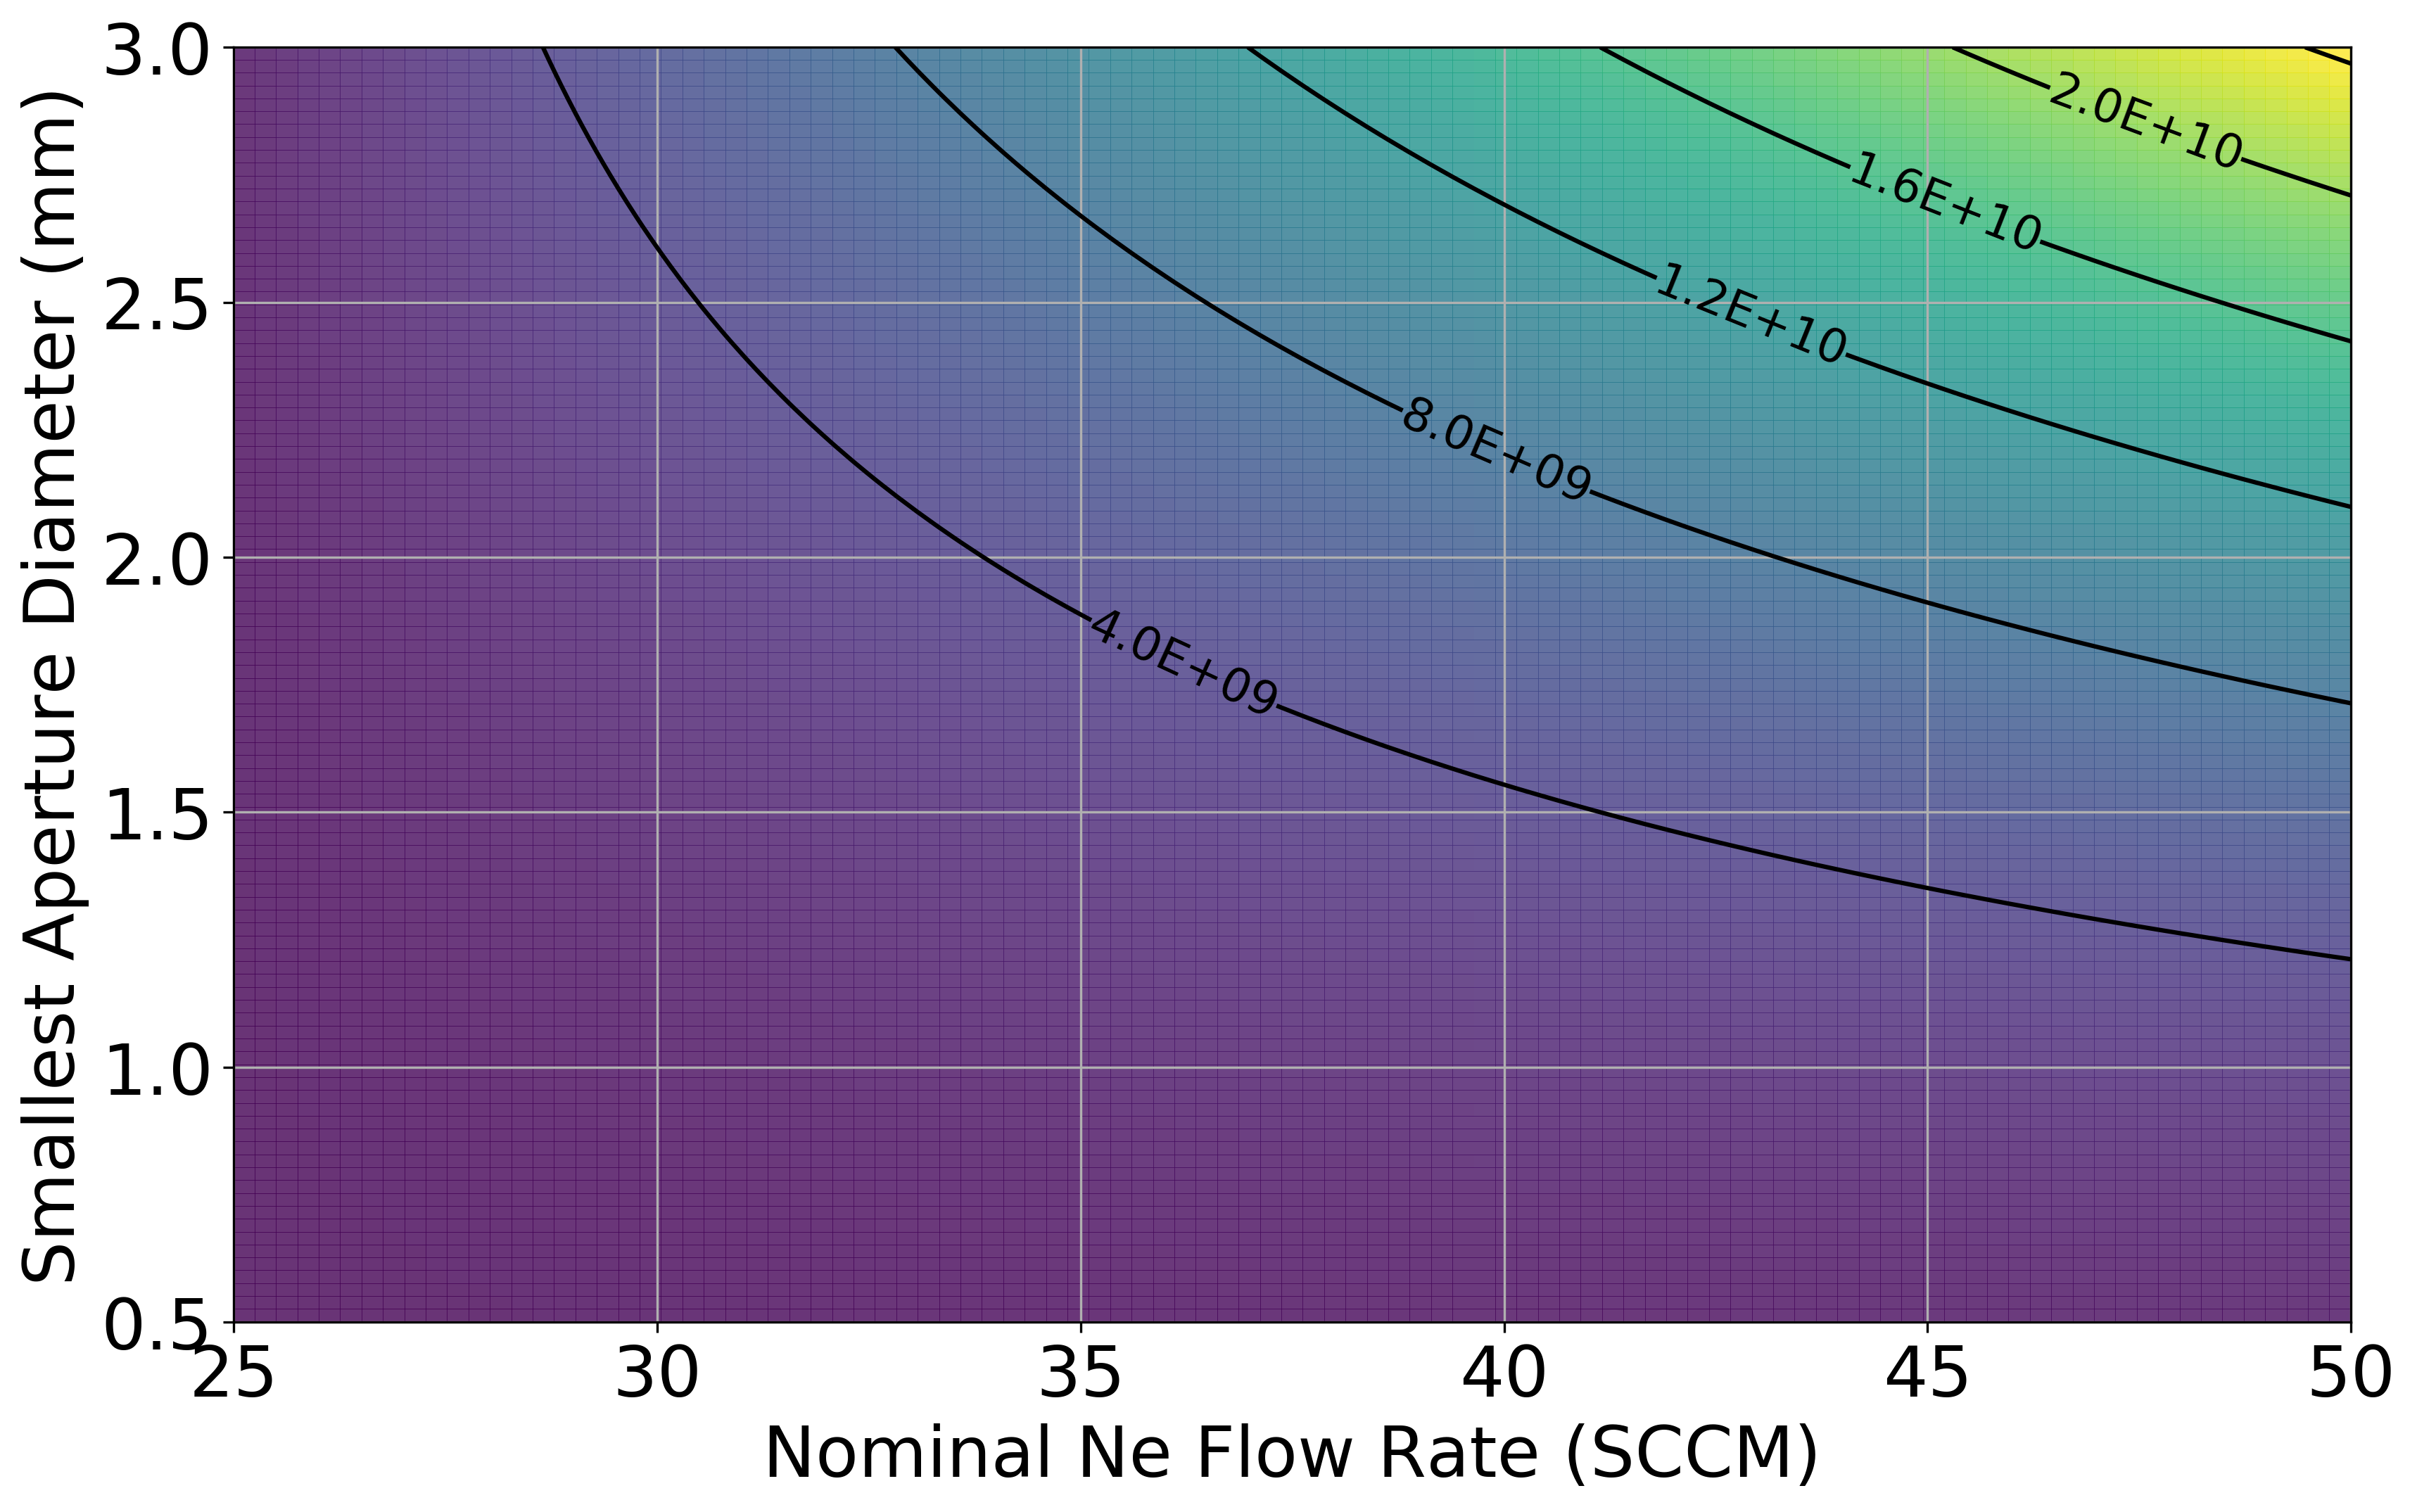
\includegraphics[width=1\textwidth]{images/CBGB_trap_density_aperture.png}
	\caption{Projected beam densities at the trap center over various nominal Ne flow rates and smallest skimmer aperture size. Beam densities shown are without throttling of the \ce{H2O} flow valve.}
	\label{fig: trap_density}
\end{figure}

One should not forget the mass dependence in the thermal velocity equation, which leads us to conclude that the choice of the species is a statement of the dominant species in the beam. If we choose to calculate the thermal velocity of the target species found in the beam due to the theoretical thermal velocity of the buffer gas, that indicates that the beam properties are still dominated by the buffer gas species. At target species/buffer gas ratios greater than 1/100, we may start to see the effects of the target species on not only the beam density, but also forward velocity.